\documentclass[conference]{IEEEtran}
\IEEEoverridecommandlockouts
% The preceding line is only needed to identify funding in the first footnote. If that is unneeded, please comment it out.
\ifCLASSOPTIONcompsoc
\usepackage[caption=false,font=normalsize,labelfont=sf,textfont=sf]{subfig}
\else
\usepackage[caption=false,font=footnotesize]{subfig}
\fi
\usepackage{cite}
\usepackage{amsmath,amssymb,amsfonts}
\usepackage{algorithmic}
\usepackage{graphicx}
\usepackage{textcomp}
\usepackage[standard]{ntheorem} 
\usepackage{longtable}
\usepackage{xcolor}
\def\BibTeX{{\rm B\kern-.05em{\sc i\kern-.025em b}\kern-.08em
    T\kern-.1667em\lower.7ex\hbox{E}\kern-.125emX}}
\usepackage{verbatim}


\begin{document}

\title{Extended State Observer Based Stator Flux Linkage Estimation of Nonlinear Synchronous Machines\\
\thanks{This work was supported by Electronics and Telecommunications Research Institute (ETRI) grant funded by the Korean government. [24ZD1160, Regional Industry ICT Convergence Technology Advancement and Support Project in Daegu-GyeongBuk (Mobility)].}
}

\author{\IEEEauthorblockN{1\textsuperscript{st} Seunghun Jang}
\IEEEauthorblockA{\textit{School of Mechanical Engineering} \\
\textit{Gwangju Institute of Science and Technology}\\
Gwangju, Republic of Korea \\
shjang7071@gm.gist.ac.kr}
\and
\IEEEauthorblockN{2\textsuperscript{nd} Bernd Pfeifer}
\IEEEauthorblockA{\textit{Laboratory for Mechatronic and Renewable Energy Systems (LMRES)
} \\
\textit{HM Munich University of Applied Sciences}\\
bernd.pfeifer@hm.edu}
\and
\IEEEauthorblockN{3\textsuperscript{rd} Christoph M. Hackl}
\IEEEauthorblockA{\textit{Laboratory for Mechatronic and Renewable Energy Systems (LMRES)
} \\
\textit{HM Munich University of Applied Sciences}\\
christoph.hackl@hm.edu}
\and
\IEEEauthorblockN{4\textsuperscript{st} Kyunghwan Choi}
\IEEEauthorblockA{\textit{School of Mechanical Engineering} \\
\textit{Gwangju Institute of Science and Technology}\\
Gwangju, Republic of Korea \\
khchoi@gm.gist.ac.kr}
}

\maketitle

\begin{abstract}
Synchronous machines (SMs) represent nonlinear dynamical systems with stator flux linkages being crucial for controller design. Among the developed methods for flux linkage estimation, the disturbance observer-based flux linkage estimator (DOB-FLE) is recognized as the state-of-the-art. However, DOB-FLE faces challenges in ensuring exponential convergence during transient conditions. To address this, this paper introduces an extended state observer-based flux linkage estimator (ESO-FLE), which represents an advancement over DOB-FLE. This novel approach utilizes extended states to model the nonlinear disturbance term as time-varying ramp signals, offering a degree of freedom compared to the constant assumption imposed for DOB-FLE and allowing for the estimation of both the extended states and the flux linkages through an ESO. Simulation results from a 35-kW SM drive demonstrate that ESO-FLE achieves exponential performance under transient conditions compared to DOB-FLE.
\end{abstract}

\begin{IEEEkeywords}
Extended state observer, disturbance observer, nonlinear synchronous machines, stator flux linkage, transient performance
\end{IEEEkeywords}

\section{Introduction}

Synchronous machines (SMs) represent dynamical systems with nonlinear stator flux linkages. Accurate knowledge of the stator flux linkages is crucial to designing high-performance controllers for SM drives. For instance, differential and secant inductance information is used to design current controllers \cite{b1,2022_Su_NonlinearCurrentControlofReluctanceSynchronousMachineswithAnalyticalFluxLinkagePrototypeFunctions} and optimal reference generators \cite{b2,2021_Hackl_GenericLossMinimizationforNonlinearSynchronousMachinesbyAnalyticalComputationofOptimalReferenceCurrentsConsideringCopperandIronLosses}, respectively. The flux linkage information itself can be utilized to predict the future behavior of the SM for model predictive control (MPC) \cite{b3}.

The stator flux linkage maps can be obtained offline through identification experiments conducted across the entire operating range \cite{b4,2022_Su_AnalyticalPrototypeFunctionsforFluxLinkageApproximationinSynchronousMachines}. However, this offline identification cannot deal with real-time parameter changes in SMs caused by aging, degradation, or abnormal operations, such as temperature rise or demagnetization.

Several studies present online estimation methods for the stator flux linkages. The stator flux linkages can be easily calculated by integrating the flux linkage dynamics defined in the $\alpha$-$\beta$ frame, but the integration results include integration errors. In \cite{b5}, a high-pass filter was applied after the integration to remove the integration errors. This method was simple and did not use any SM parameter information, but the filter distorted the frequency response, particularly in the low-frequency region. 
Another simple online estimation method is to adopt the steady-state assumption for the flux linkage dynamics defined in the rotating $d$-$q$ frame and to calculate the flux linkages directly from the steady-state model \cite{b6}, \cite{b7}. The high-frequency current injection has recently been adopted for the stator flux linkage estimation \cite{b8} and has shown satisfactory steady-state performance. However, these approaches could not guarantee sufficient transient performance. Using a state observer, such as sliding mode observers \cite{b9} or extended Kalman filters \cite{b10}, was also proposed for online flux linkage estimation, but these observers were designed based on prior knowledge of machine parameters, which is difficult to obtain without accurate knowledge of the stator flux linkages.

Recently, online flux linkage estimators have been proposed, which do not require accurate knowledge of machine parameters but provide remarkable estimation performance. In \cite{b11}, a disturbance observer-based flux linkage estimator (DOB-FLE) was proposed, which could estimate the flux linkages without knowing the accurate value of the inductance matrix, with the help of the DOB estimating the nonlinear disturbance term. An advanced $\alpha$-$\beta$ frame-based estimator was presented in \cite{b12}, where integration errors were estimated by a linear state observer and compensated for in the time domain, which differed from using a frequency-domain approach. Both methods presented in \cite{b11} and \cite{b12} offered remarkable estimation performance even using inaccurate nominal machine parameters. However, they struggled with ensuring exponential convergence during transient states, and their transient performance deteriorated when using nominal parameters that differ significantly from the true parameters.

With this background, this paper presents an extended state observer-based flux linkage estimator (ESO-FLE), an advancement over DOB-FLE with improved transient performance. The key difference between the proposed ESO-FLE and DOB-FLE is that ESO-FLE introduces extended states to model the nonlinear disturbance term as time-varying
ramp signals, in contrast to the constant assumption used in DOB-FLE. By doing so, both flux linkages and extended states can be estimated more accurately via an ESO. The effectiveness of the proposed ESO-FLE is numerically validated using a 35-kW interior permanent magnet synchronous machine (IPMSM). 

\section{Preliminaries}
\subsection{Nonlinear Synchronous Machine Model}
%
The SM is modeled in the rotating $d$-$q$ frame as follows~\cite{b13}:
    \begin{align}\label{eqn:se_dq}
    {\dot{\boldsymbol{{{\lambda}}} }_{dq}(t)} &= {{\boldsymbol{v}}_{dq}(t)} - {{{R}}_{s}} {\boldsymbol{i}}_{dq}(t) -\omega_{r}\boldsymbol{J} { {\boldsymbol{{\lambda}} }_{dq}(t)},
    \end{align}   
 with ${{\boldsymbol{z}}_{dq} :=\begin{bmatrix} {z}_{d} & {z}_{q}\end{bmatrix}^{T}}$, $z = {{{{\lambda}}} }, {{v}},{{i} } $, stator flux linkages ${\boldsymbol{\lambda}}_{dq}$, stator voltages $ {\boldsymbol{v}}_{dq}$, stator currents $ { {\boldsymbol{i}} }_{dq}$, stator winding resistance $R_s$, rotation matrix ${ {\boldsymbol{J}}:=\begin{bmatrix}\notag 0 & -1 \\ 1 & 0 \end{bmatrix} }$, and electrical rotor speed $\omega_r$. The nonlinear flux linkages are generally modeled by a nonlinear function of the stator currents as ${\boldsymbol{\lambda}_{dq}}(t) = \boldsymbol{f}({\boldsymbol{i}_{dq}}(t))$.

The following assumptions are imposed:
    \begin{itemize}
    \item The stator winding resistance $R_s$ is accurately known.
    \item The inverter nonlinearity and iron loss in the electrical dynamics are neglected.
    \item The electrical rotor speed $\omega_r$ varies slowly compared to the electrical quantities (e.g. currents or flux linkages).
    \end{itemize}
    
\subsection{Disturbance Observer-Based Stator Flux Linkage Estimator (DOB-FLE)} 

DOB-FLE, presented in \cite{b11}, is based on the idea of separating the nonlinear flux linkages into a linear term ${\boldsymbol{L}_{s,0}}{\boldsymbol{i}}_{dq}$ and a nonlinear disturbance term $\Delta_{\boldsymbol{\lambda}_{dq}}$ as follows:     \begin{align}\label{eqn:flx_dq}
    {\boldsymbol{\lambda}_{dq}}(t) = {\boldsymbol{L}_{s,0}}{\boldsymbol{i}}_{dq}(t) + \Delta_{\boldsymbol{\lambda}_{dq}}(t),
    \end{align}
which can be rearranged as follows 
    \begin{align}\label{eqn:flx_dq_re}
    {\boldsymbol{i}}_{dq}(t)&={\boldsymbol{L}_{s,0}}^{-1}\left( {\boldsymbol{\lambda}_{dq}}(t) -\Delta_{\boldsymbol{\lambda}_{dq}}(t)\right), 
    \end{align}    
where ${\boldsymbol{L}_{s,0}}$ denotes a constant nominal inductance matrix. 

The following state-space model is obtained by substituting \eqref{eqn:flx_dq_re} into the nonlinear flux linkage dynamics (\ref{eqn:se_dq}), i.e.   
\begin{align}\label{eqn:sota_eq}
    \begin{cases}
    {\dot{\boldsymbol{{{\lambda}}} }_{dq}(t)} = {{\boldsymbol{v}}_{dq}(t)} - {{{R}}_{s}} {\boldsymbol{L}_{s,0}}^{-1}\left( {\boldsymbol{\lambda}_{dq}}(t) - \Delta_{\boldsymbol{\lambda}_{dq}}(t)\right) \\ 
    \quad\quad\quad\quad\ - \omega_{r}\boldsymbol{J} { {\boldsymbol{{\lambda}} }_{dq}(t)} \\
    \dot \Delta_{\boldsymbol{\lambda}_{dq}}(t) = 0 \\
   {\boldsymbol{i}}_{dq}(t) = {\boldsymbol{L}_{s,0}}^{-1}\left( {\boldsymbol{\lambda}_{dq}}(t) -\Delta_{\boldsymbol{\lambda}_{dq}}(t)\right), 
    \end{cases}
    \end{align}
with $\boldsymbol{{{\lambda}}}_{dq}$ and $\Delta_{\boldsymbol{\lambda}_{dq}}$ as states, ${{\boldsymbol{v}}_{dq}}$ as inputs, and ${\boldsymbol{i}}_{dq}$ outputs. This model is observable as shown in \cite{b11}. The linear state observer was designed in \cite{b11} to estimate the full states asymptotically (in steady state). 

However, this model assumes $\dot \Delta_{\boldsymbol{\lambda}_{dq}}(t) = 0$ (i.e., $\Delta_{\boldsymbol{\lambda}_{dq}}(t)$ is constant), which is only true in the steady state because the disturbance term, defined by 
\begin{align}
\Delta_{\boldsymbol{\lambda}_{dq}}(t) := {\boldsymbol{\lambda}_{dq}}(t)(=\boldsymbol{f}({\boldsymbol{i}_{dq}}(t))) - {\boldsymbol{L}_{s,0}}{\boldsymbol{i}}_{dq}(t), 
\end{align}  
is a function of the stator currents. Therefore, the flux linkage estimation cannot converge during transient states and even may have a large transient error when using an inaccurate nominal inductance matrix, as the nonzero $\dot \Delta_{\boldsymbol{\lambda}_{dq}}(t)$ term acts as a time-varying external quantity.

\section{Extended State Observer-based Flux Linkage Estimator (ESO-FLE)}

This section presents ESO-FLE, which is an improved version of DOB-FLE with enhanced transient performance. The key idea is to assign non-constant dynamics for $\Delta_{\boldsymbol{\lambda}_{dq}}$ by introducing an (additional) extended state. 

\subsection{Extended State-Space Model}\label{subsec:dy_mdl}
%
The extended states $\boldsymbol{l}_{dq}$ is added to the nonlinear disturbance dynamics as follows  
    \begin{align}\label{eqn:rp_dob}
    \begin{cases}
    \boldsymbol{\dot \Delta}_{\boldsymbol{\lambda}_{dq}}(t) =     
    \boldsymbol{l}_{dq}(t) \\
      \boldsymbol{\dot l}_{dq}(t) = 0.
      \end{cases}
    \end{align} 
The extended states are regarded as constant terms, thereby making the nonlinear disturbance terms behave like ramp signals with constant slopes. This model is more flexible than regarding the nonlinear disturbance term as constant.

An extended state-space model is obtained by replacing the nonlinear disturbance dynamics in \eqref{eqn:sota_eq} with \eqref{eqn:rp_dob}, i.e.
\begin{align}\label{eqn:ss_mdl}
    \begin{cases}
    {{\boldsymbol{{\dot {x}}} }(t)}={{\boldsymbol{A}}({\omega}_{r}(t))} {{\boldsymbol{x}}(t)} + {{\boldsymbol{B}}{\boldsymbol{u}}(t)}\\
    {\boldsymbol{y}(t)} = {{\boldsymbol{C}}} {{\boldsymbol{x}(t)}}
    \end{cases}
    \end{align}
with 
     \begin{align}\notag
        {\boldsymbol{x}} &:= \begin{bmatrix}
        {\boldsymbol{\lambda}_{dq}}  & \boldsymbol{\Delta}_{\boldsymbol{\lambda}_{dq}} & \boldsymbol{l}_{dq}
        \end{bmatrix}^T, \\\notag
        {{\boldsymbol{A}}({\omega}_{r}(t))} &:= \begin{bmatrix}
        - {{{R}}_{s}} {\boldsymbol{L}_{s,0}}^{-1} - \omega_{r}(t)\boldsymbol{J} & {{{R}}_{s}} {\boldsymbol{L}_{s,0}}^{-1}  & {\boldsymbol{O}}_{2\times2} \\ 
        {\boldsymbol{O}}_{2\times2} & {\boldsymbol{O}}_{2\times2} & {\boldsymbol{I}}_{2} \\
        {\boldsymbol{O}}_{2\times2} & {\boldsymbol{O}}_{2\times2} & {\boldsymbol{O}}_{2\times2}
        \end{bmatrix},
        \\\notag
        {\boldsymbol{B}} &:= \begin{bmatrix}
        {\boldsymbol{I}}_{2} \\ 
        {\boldsymbol{O}}_{2\times2} \\
        {\boldsymbol{O}}_{2\times2} 
        \end{bmatrix},        
        {\boldsymbol{C}} := \begin{bmatrix}
        {\boldsymbol{L}_{s,0}}^{-1} & -{\boldsymbol{L}_{s,0}}^{-1} & {\boldsymbol{O}}_{2\times2}
        \end{bmatrix},
    \end{align} 
where ${\boldsymbol{x}}$ denotes the state vector, and, ${{\boldsymbol{A}}({\omega}_{r})}$, ${\boldsymbol{B}}$ and ${\boldsymbol{C}}$ represent the system, input and output matrices, respectively.
To analyze whether the states of system \eqref{eqn:ss_mdl} are fully observable, the observability matrix is analyzed (for constant $\omega_r$), i.e.
    \begin{align}\label{eqn:osv}
    {\boldsymbol{\mathcal{O}}(\omega_{r})} &= \begin{bmatrix} 
    {\boldsymbol{C}}\\\boldsymbol{C}{{\boldsymbol{A}}({\omega}_{r})}\\\boldsymbol{C}{{\boldsymbol{A}}({\omega}_{r})}^2 \\\boldsymbol{C}{{\boldsymbol{A}}({\omega}_{r})}^3  
    \end{bmatrix},
    \end{align}
which is evaluated using the first three rows of ${\boldsymbol{\mathcal{O}}(\omega_{r})}$ for the simplicity. Consequently, the observability matrix has full rank (i.e., ${\boldsymbol{\mathcal{O}}(\omega_{r}}$) = 6) if ${\omega}_{r} \neq 0$, and the state $\boldsymbol{x}$ is (locally) fully observable.

\begin{comment}
[Reviewer 1]

Here are some comments: 

1. I would suggest to change A, B ,C and x with machine parameters.

2. The whole control system diagram is missing 

3. in Fig.2, why the flux d is decreasing with the increasing of torque?? 

4. in Fig.3, it seems for the spikes have certain fix frequency? Why it is that? 

5. the base speed is 2000rpm, but the simulation can only reach 1200rpm? It seems there is only no load test shown, the sudden loadup test is needed.

[Reviewer 2]

The paper proposed the ESO for flux linkage estimation, focusing on accurate estimation during transient states. It is interesting and well-structured; please consider the following comments: 

- 1. it would be more informative to provide information for the selection of the feedback gain matrix F; 

- 2. adding a block diagram of the proposed ESO-FLE can be helpful for readers; 

- 3. as the IPMSM is used as a study case, why are the values for d-axis and q-axis inductances equal? 

- 4. in Fig.3, it is better to select different colours for the ESO-FLE and DOB-FLE to highlight the difference; 

 -5. "DOB-FLM" instead of "DOB-FLE" on page 3.
\end{comment}

\subsection{Extended State Observer Design}\label{subsec:ss_obs}

A linear (time-varying) extended state observer for the model (\ref{eqn:ss_mdl}) is designed as follows
    \begin{align}\label{eqn:ob_eq}
    \begin{cases}
    {{{{\dot {\hat{\boldsymbol{x}}}}}}(t)}=  {{\boldsymbol{A}}({\omega}_{r}(t))}{\hat{\boldsymbol{{x}}}(t)} + {\boldsymbol{B}}{\boldsymbol{u}}(t) + {{\boldsymbol{F}}}({\boldsymbol{y}}(t) - {\hat{\boldsymbol{{y}}}} (t))\\
    {\hat{\boldsymbol{{y}}}}(t) = {{\boldsymbol{C}}} {{\hat{\boldsymbol{{x}}}}}(t),
    \end{cases}
    \end{align}
where ${\hat{\boldsymbol{{x}}}}$ and ${\hat{\boldsymbol{{y}}}}$ represent the estimates of ${\boldsymbol{{x}}}$, and ${\boldsymbol{{y}}}$ and ${{\boldsymbol{F}}}$ is the feedback gain matrix dependent on the electrical angular rotor velocity $\omega_r$. The estimation error dynamics are obtained by subtracting (\ref{eqn:ob_eq}) from (\ref{eqn:ss_mdl}) leading to  
    \begin{align}    
    {{\boldsymbol{{\dot {e}}} }}(t)=\left[ {{\boldsymbol{A}}({\omega}_{r})} - {{\boldsymbol{F}}}{{\boldsymbol{C}}}\right] {\boldsymbol{{e}}}(t),
    \end{align} 
where ${{\boldsymbol{e}} } := {{\boldsymbol{x}} } -  {{\boldsymbol{\hat x}} }$ denotes the estimation error. If the matrix ${{\boldsymbol{A}}({\omega}_{r})} - {{\boldsymbol{F}}} {{\boldsymbol{C}}}$ is Hurwitz (with eigenvalues having negative real parts), the estimation error will converge exponentially to zero (for constant $\omega_r$). To determine the observer gain matrix ${{\boldsymbol{F}}}$ for a MIMO system, a robust pole assignment method \cite{b14} is utilized to place the system poles at the desired (stable) eigenvalues, which can be easily achieved by using the MATLAB command \texttt{"place"} to calculate the gain matrix ${{\boldsymbol{F}}}$.

\begin{figure}[!t]
    \centering
    \captionsetup{font=footnotesize}
    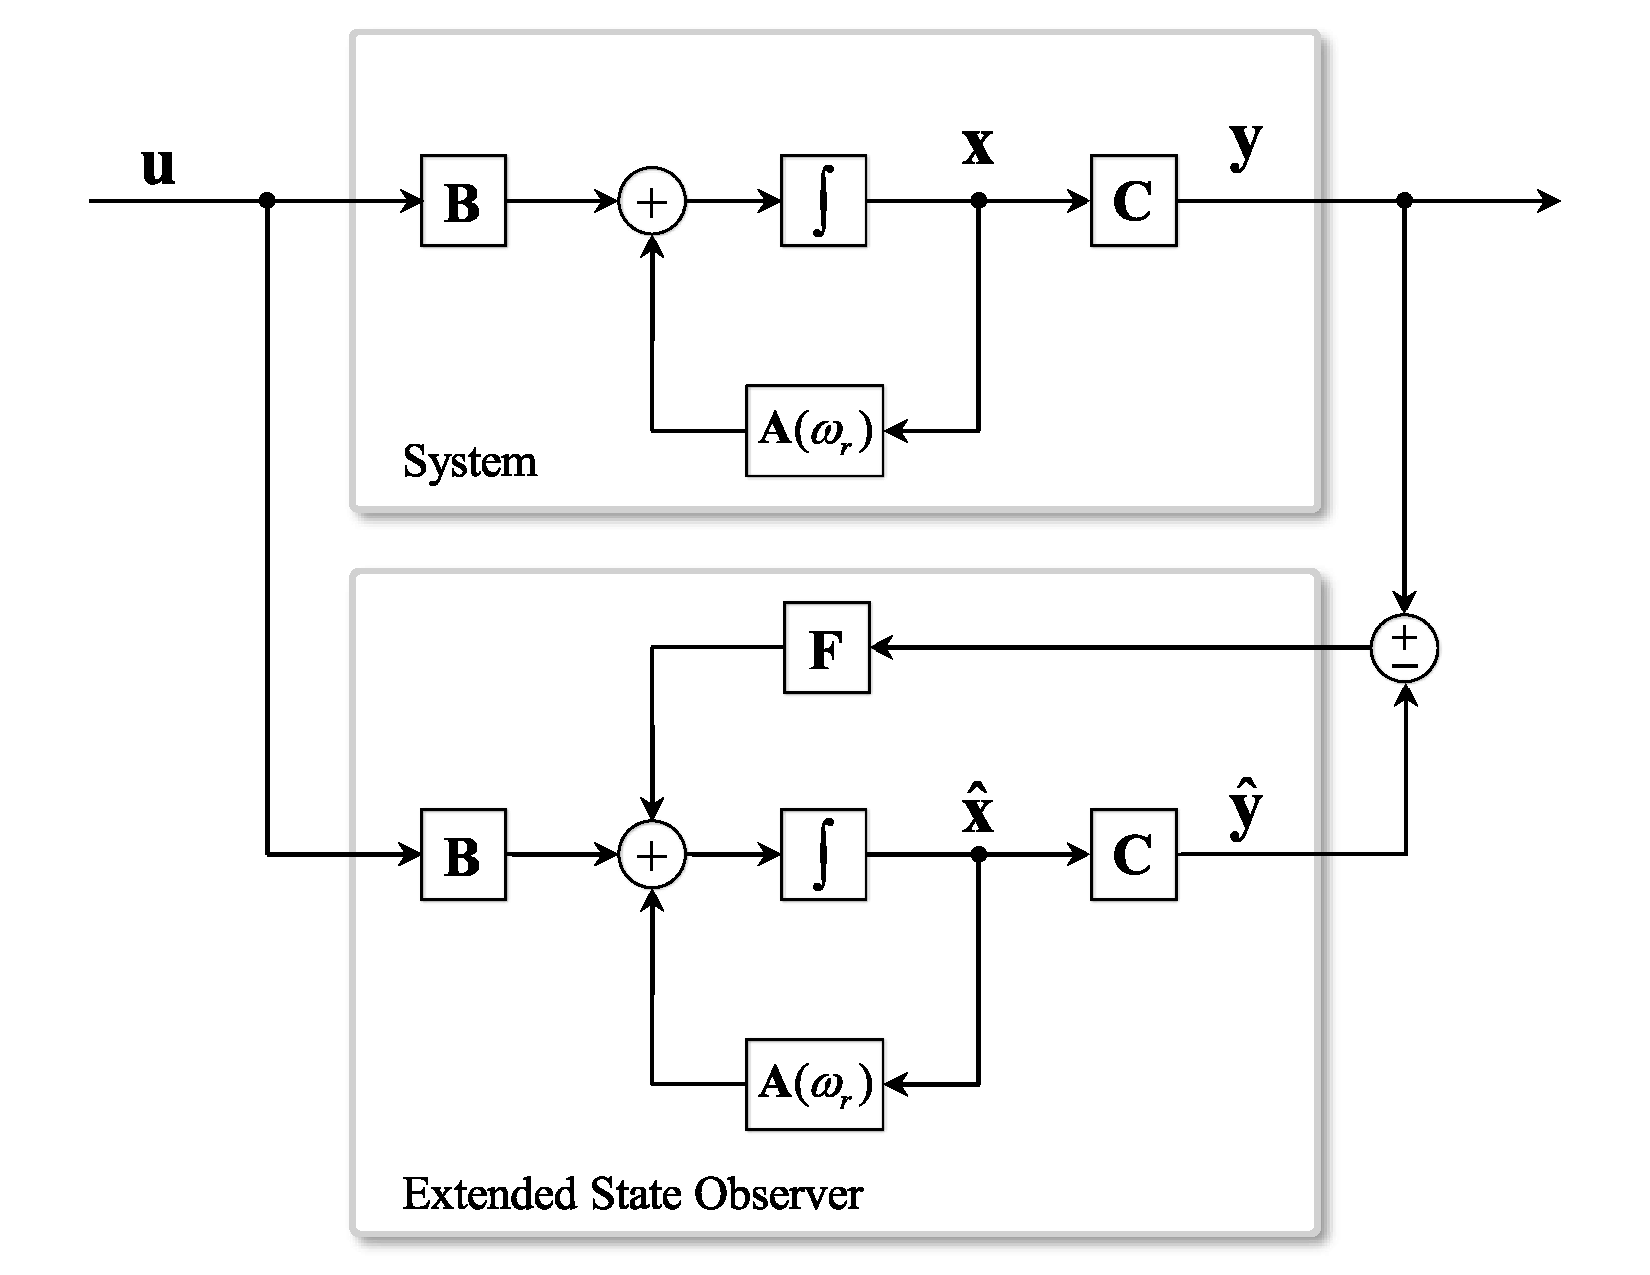
\includegraphics[width=0.9\columnwidth ]{Fig1_1.pdf}
    \caption{Observer block diagram for the proposed ESO-FLE.}\label{Fig1}
\end{figure}

\begin{table}
\caption{Specifications of the IPMSM Drive}\label{Tab1}
\centering
\begin{tabular}{l r}\hline
\textbf{Parameter} & \textbf{Value}  \\ \hline
Base speed & 2000 rpm \\
Maximum torque & 180 Nm\\
DC-link voltage  & 325 V \\
Maximum stator current  & 350 A \\
Rotor Inertia & 0.1234 kg\,m$^2$ \\
Number of pole pairs & 8\\
Stator winding resistance ($R_s$) & 10.9 m$\Omega$\\\hline
\end{tabular}
\end{table}

\begin{figure}
    \centering
    \captionsetup{font=footnotesize}
    \subfloat[]{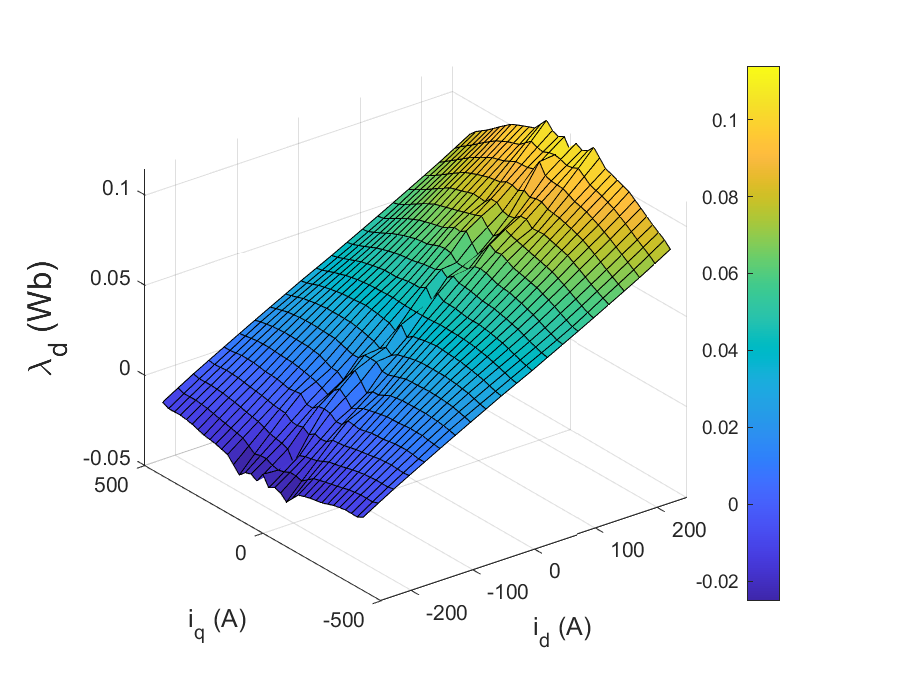
\includegraphics[width=0.49\linewidth]{Fig3_a.eps}}\label{fig:subfig3-a}
    \hfill
    \subfloat[]{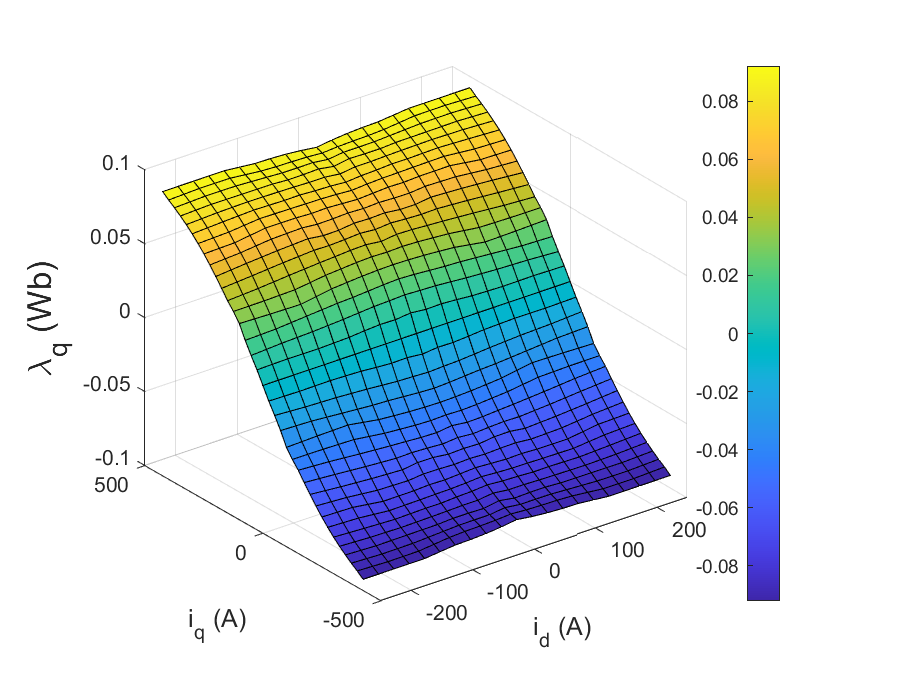
\includegraphics[width=0.49\linewidth]{Fig3_b.eps}}\label{fig:subfig3-b}
    \caption{Nonlinear flux linkage maps of the IPMSM. (a) $d$-axis and (b) $q$-axis.}
    \label{Fig3}
\end{figure}

\section{Validation}

\subsection{Setup}
The proposed ESO-FLE was validated using MATLAB/ SIMULINK simulation, built based on the `\texttt{Three-phase PMSM Traction Drive}' example provided by MathWorks.
A 35-kW IPMSM drive, whose specifications and flux linkage maps are listed in Table \ref{Tab1} and shown in Fig. \ref{Fig3}, respectively, was controlled by finite control set MPC \cite{b15} to track the $d$-$q$ axis current references, respectively. The numerical reference generator presented in \cite{b16} was utilized to convert a torque command into current references using lookup table data for the $d$-$q$ axis inductances ($L_d$, $L_q$) and the permanent magnetic flux linkages ($\Psi_m$) of the synchronous machine. The overall control block diagram and state observer are shown in Fig. \ref{Fig3}. The feedback gain matrix ${{\boldsymbol{F}}}$ was designed to make the (stable) eigenvalues of matrix ${{\boldsymbol{A}}({\omega}_{r})} - {{\boldsymbol{F}}} {{\boldsymbol{C}}}$ became 628 rad/s at a mechanical speed of 500 RPM. The bandwidth of the desired eigenvalues was selected to be approximately 100 Hz, which is about twice as large as the settling time (50 Hz) of the torque reference command, considering the estimation performance.
 \begin{figure*}
    \centering
    \captionsetup{font=footnotesize}
    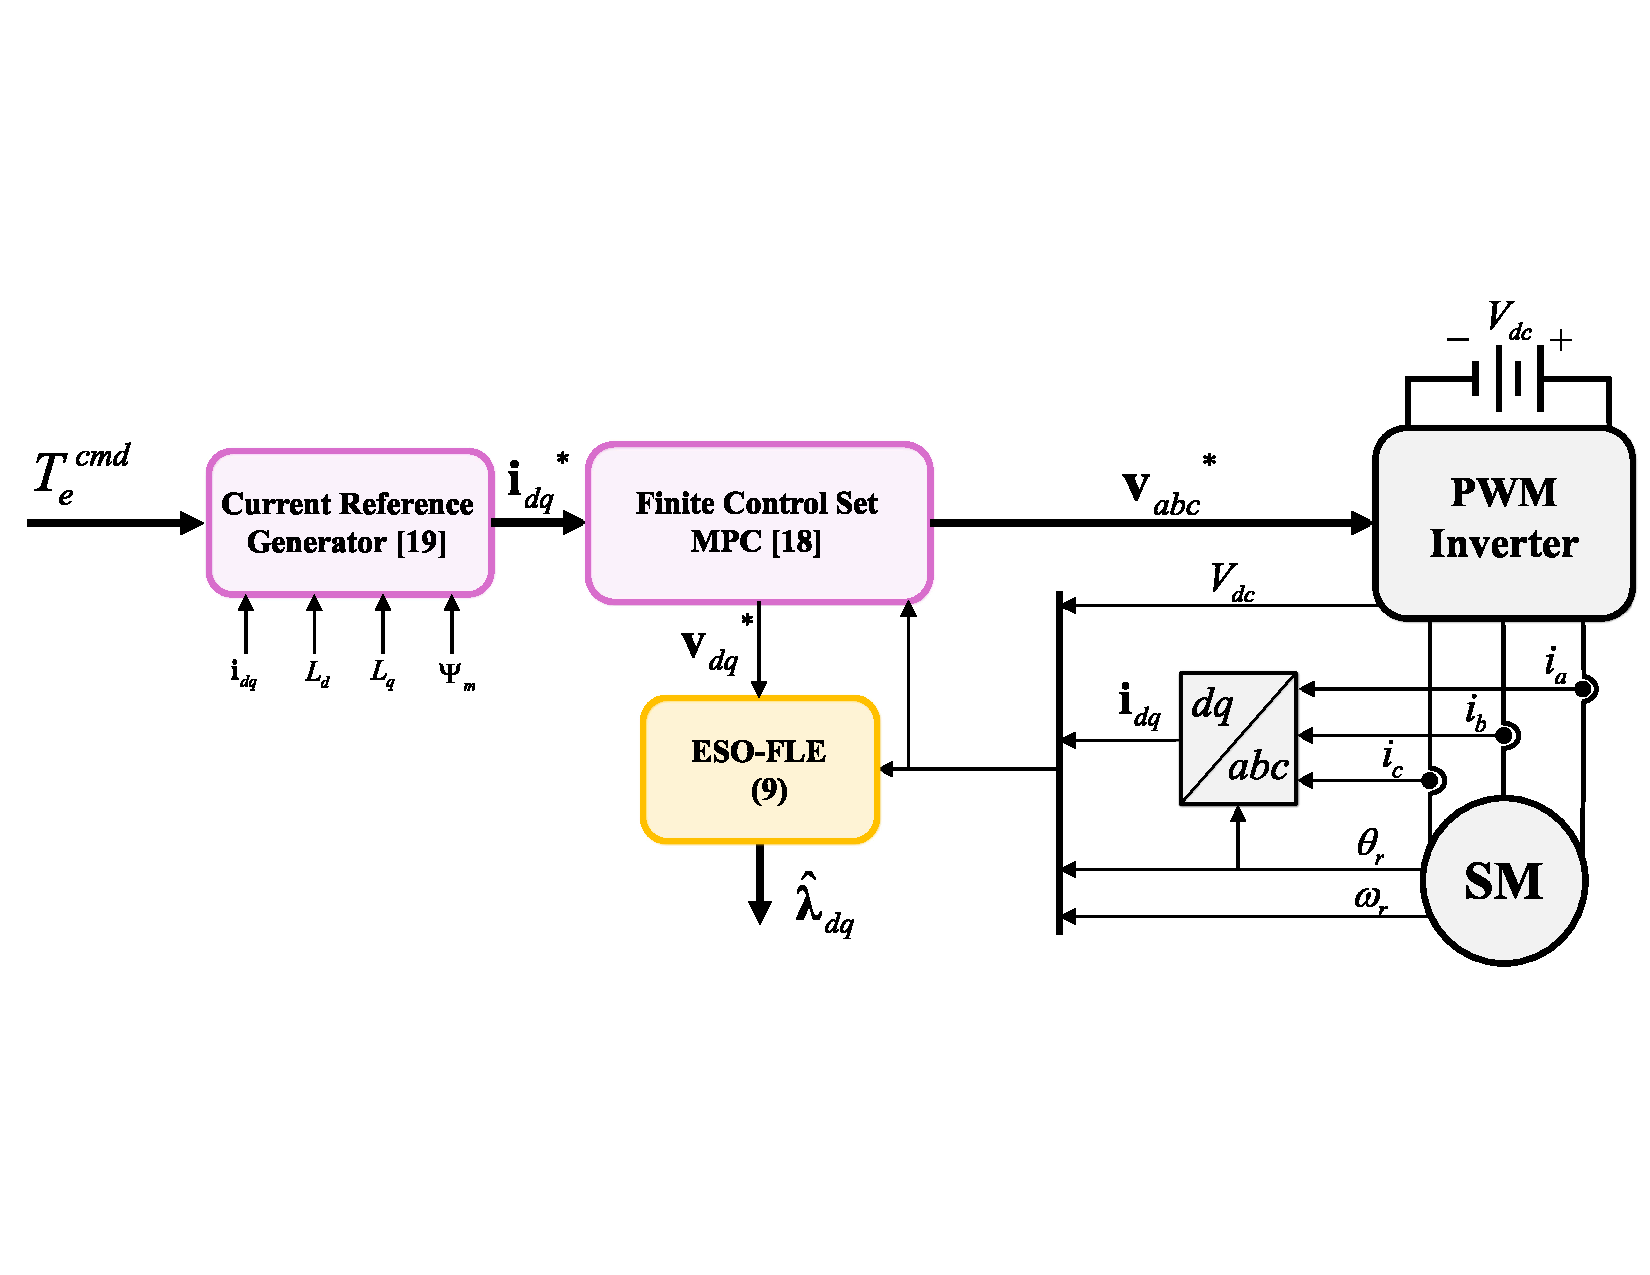
\includegraphics[width=1.4 \columnwidth ]{Fig3_1.pdf}
    \caption{Control block diagram.}\label{Fig3}
 \end{figure*}
 
The simulative validation consists of two parts. For the first part (see Section \ref{sec_a}), the performance of the proposed ESO-FLE was examined while controlling the torque ranging from -180 to 180 Nm within a mechanical speed range from 200 to 1300 RPM. The nominal inductance matrix, which can be chosen 
arbitrarily, is defined by the secant inductance values along the $d$-$q$ axis at zero current, placed as diagonal elements, with all off-diagonal elements set to zero (i.e., ${\boldsymbol{ {L}}}_{s,0}  = {\tiny \begin{bmatrix} 0.28 & 0 \\ 0 & 0.28 \end{bmatrix}}$mH). 
For the second part (see 
Section \ref{sec_b}), ESO-FLE was compared with DOB-FLE, under the condition that a torque command increased from 0 to 180 Nm within 0.02 s at a mechanical speed of 500 RPM. The feedback gain matrix of DOB-FLE was also selected so that it had the same eigenvalues at 500 RPM as ESO-FLE. The nominal inductance matrix was set to ${\boldsymbol{ {L}}}_{s,0}  = {\tiny \begin{bmatrix} 0.14 & 0 \\ 0 & 0.14 \end{bmatrix}}$mH, which is half of the value defined in the first part, for both ESO-FLE and DOB-FLE to simulate an adverse scenario.
 
\begin{figure}[!t]
    \centering
    \captionsetup{font=footnotesize}
    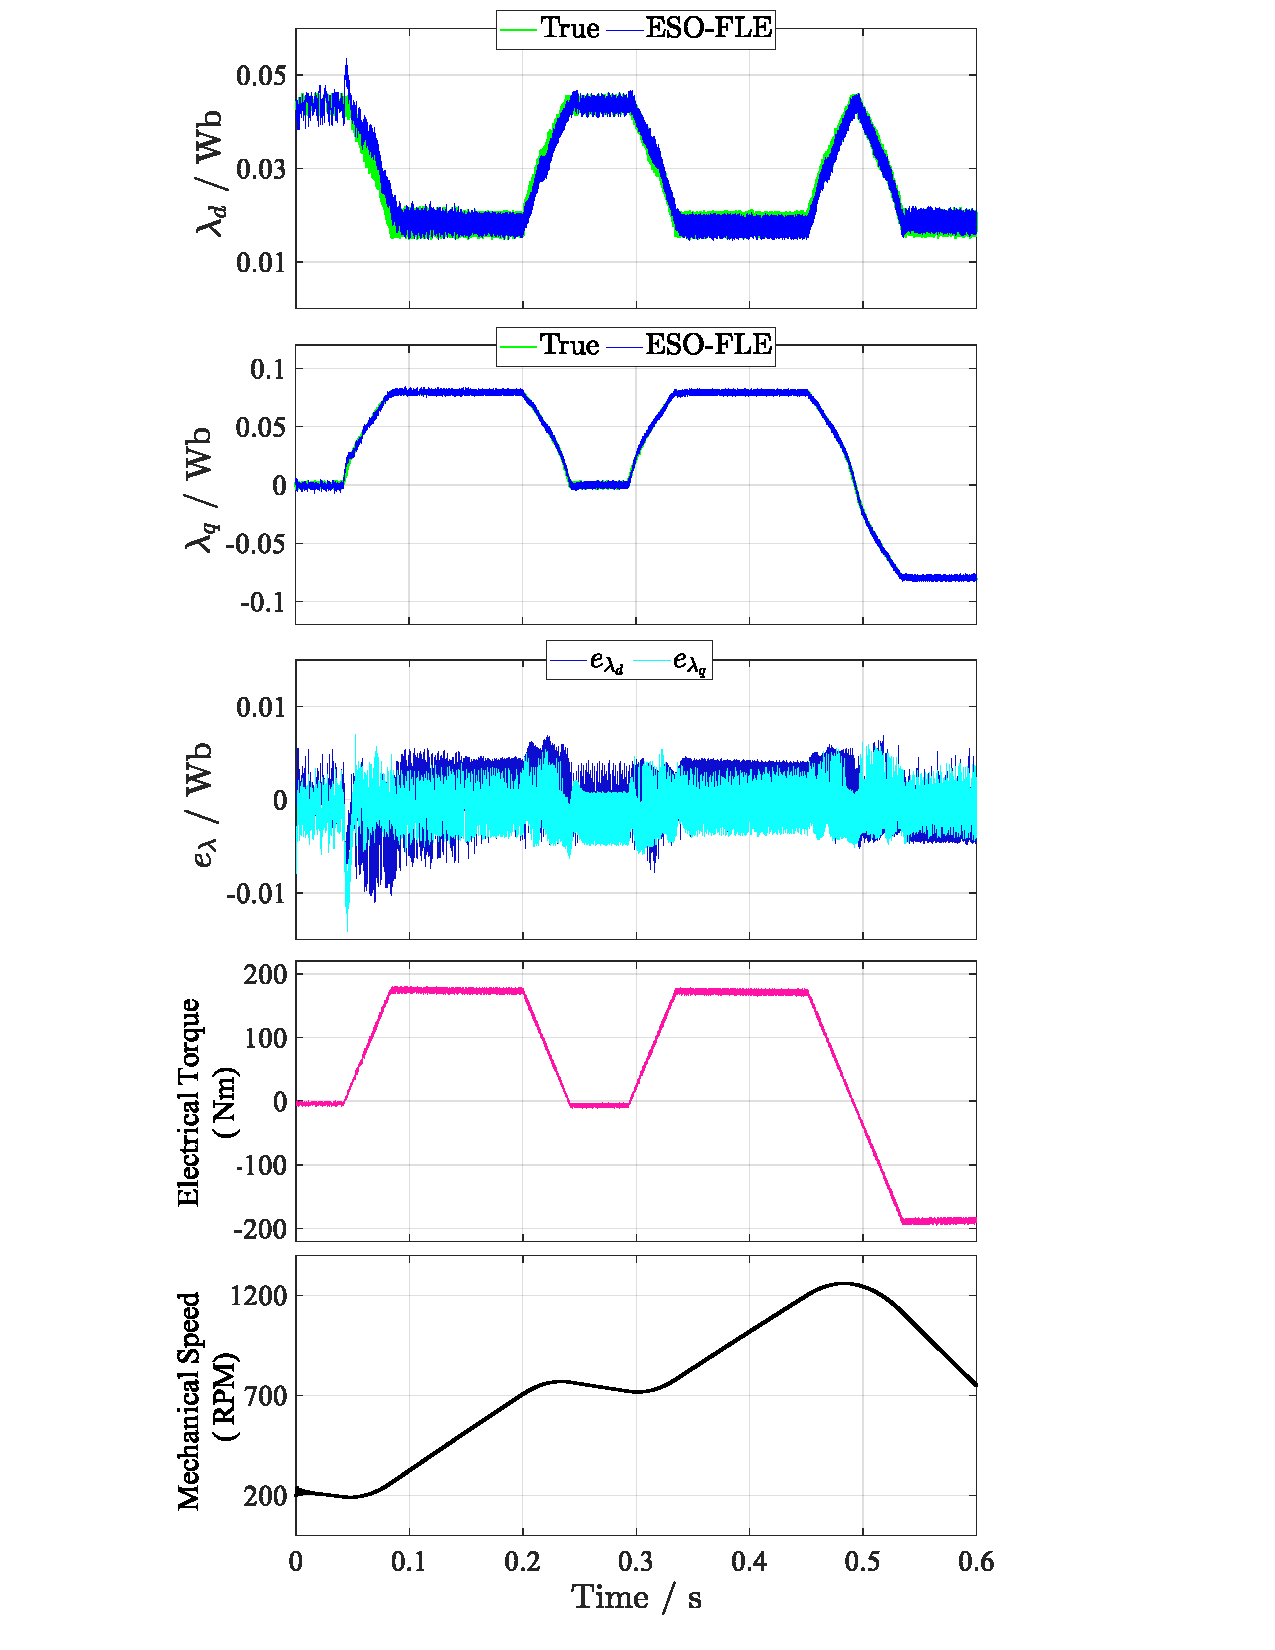
\includegraphics[width=0.9\columnwidth ]{Fig4.pdf}
    \caption{Flux linkage estimates of the proposed ESO-FLE.}\label{Fig4}
\end{figure}

\subsection{Validation of the Proposed ESO-FLE}\label{sec_a}

\begin{figure}[!t]
    \centering
    \captionsetup{font=footnotesize}
    \subfloat[]{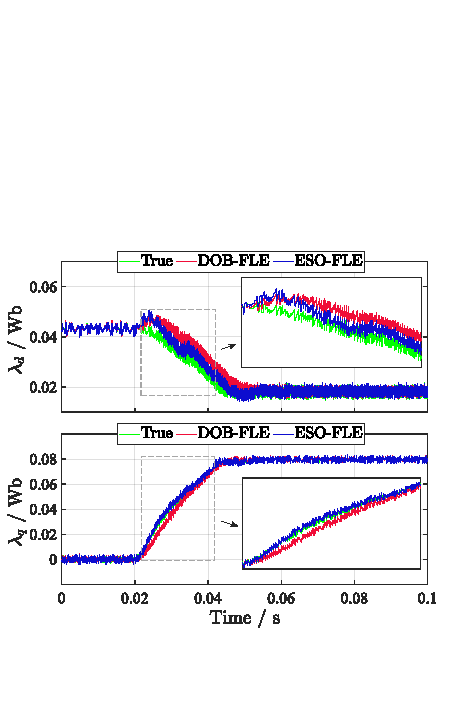
\includegraphics[width=0.9\columnwidth ]{Fig5_a.pdf}}\label{fig:subfig5-a}\\
    \subfloat[]{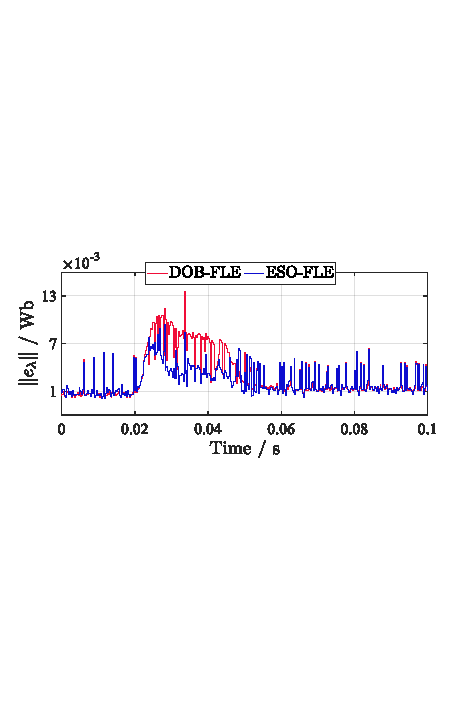
\includegraphics[width=0.9\columnwidth ]{Fig5_b.pdf}}\label{fig:subfig5-b}
    \caption{Comparison of the proposed ESO-FLE and DOB-FLE. (a) Flux linkage estimates. (b) The corresponding estimation error norm $ \| \boldsymbol{e}_{\lambda} \|$.}\label{Fig5}
\end{figure}
    
Figure \ref{Fig4} shows the flux linkage estimates, their estimation errors ${\boldsymbol{e}_{\lambda} := \boldsymbol{\lambda}_{dq} - \boldsymbol{\hat\lambda}_{dq}}$, and the operating conditions for the proposed ESO-FLE. At $t=0.05$  seconds, when the torque command starts increasing to 180 Nm, a large spike-like estimation error occurs during the transient states. This is because the observer gain matrix ${{\boldsymbol{F}}}$ was designed for a constant speed of 500 rpm, causing the observer gain to be sensitive in the low-speed region, affecting the estimation performance. Above 200 RPM, the flux linkage estimates closely tracked their true values under dynamic operating conditions across a wide operating range of torque and speed. The estimation error was nearly identical in both transient and steady states, suggesting that incorporating the extended state into the state-space model effectively enhanced the transient estimation performance.

\subsection{Comparison of ESO-FLE and DOB-FLE}\label{sec_b}
    
Figure \ref{Fig5}a shows the simulation results for the comparison between ESO-FLE and DOB-FLE, demonstrating that ESO-FLE exhibits an improved transient performance compared to DOB-FLE. This enhancement can be attributed to ESO-FLE's approach of treating the nonlinear disturbance term as time-varying ramp signals, unlike DOB-FLE which assumes these disturbances to be constants. 

Figure \ref{Fig5}b shows the estimation error norm $ \| \boldsymbol{e}_{\lambda} \|$ between ESO-FLE and DOB-FLE, representing the quantitative estimation performance. Because the finite control set MPC method directly determined the $d$- and $q$-axis voltage references for the $d$- and $q$-axis current references, respectively, it seems that both ESO-FLE and DOB-FLE included significant switching ripples in their estimation error norms. However, it is evident that only the estimation error of ESO-FLE decreased during transient states. Consequently, it is demonstrated that the proposed method performs well in both steady and transient states even with inaccurate nominal inductance.

\section{Conclusion}

This paper introduced ESO-FLE, an enhanced version of DOB-FLE, with the latter recognized as the state-of-the-art method for online flux linkage estimation. The main contribution was introducing extended states to accurately model the nonlinear flux linkage dynamics, treating the nonlinear disturbance term as time-varying ramp signals. This differs from DOB-FLE,  which treats the nonlinear disturbance term as constants. Simulation results using a 35 kW IPMSM drive demonstrated that ESO-FLE outperformed DOB-FLE during transient conditions for flux linkage estimation under varying operating conditions. Future research will focus on experimental validation of the proposed method, with a particular emphasis on addressing non-ideal factors such as inverter nonlinearities.

\begin{thebibliography}{00}
\bibitem{b1} Antonello, Riccardo, et al. "Advanced current control of synchronous reluctance motors." {\it{2017 IEEE 12th International Conference on Power Electronics and Drive Systems (PEDS).}} IEEE, 2017.
\bibitem{2022_Su_NonlinearCurrentControlofReluctanceSynchronousMachineswithAnalyticalFluxLinkagePrototypeFunctions} 
Shih-Wei Su, Hannes B{\"o}rngen, Christoph M. Hackl and Ralph Kennel, "Nonlinear Current Control of Reluctance Synchronous Machines With Analytical Flux Linkage Prototype Functions"
{\it {IEEE} Open Journal of the Industrial Electronics Society}, 2022 (doi: 10.1109/OJIES.2022.3208329).
\bibitem{b2} Anian Brosch, Oliver Wallscheid, and Joachim Böcker. "Torque and inductances estimation for finite model predictive control of highly utilized permanent magnet synchronous motors." {\it{IEEE Transactions on Industrial Informatics}} 17.12 (2021): 8080-8091. 
\bibitem{2021_Hackl_GenericLossMinimizationforNonlinearSynchronousMachinesbyAnalyticalComputationofOptimalReferenceCurrentsConsideringCopperandIronLosses} 
Christoph M. Hackl,  Julian Kullick and Niklas Monzen, "Generic loss minimization for nonlinear synchronous machines by analytical computation of optimal reference currents considering copper and iron losses"
{\it 2021 {IEEE} International Conference on Industrial Technology ({ICIT})}, 2021 (doi: 10.1109/icit46573.2021.9453497).
\bibitem{b3} Wendel, Sebastian, et al. "Flux linkage-based direct model predictive current control for synchronous machines." {\it{IEEE Transactions on Power Electronics}} 36.12 (2021): 14237-14256.
\bibitem{b4} E. Armando, R. I. Bojoi, P. Guglielmi, G. Pellegrino, and M. Pastorelli, “Experimental identification of the magnetic model of synchronous machines,” {\it{IEEE Transactions on Industry Applications}}, vol. 49, no. 5, pp. 2116-2125, 2013. 
\bibitem{2022_Su_AnalyticalPrototypeFunctionsforFluxLinkageApproximationinSynchronousMachines}
Shih-Wei Su,  Christoph M. Hackl and Kennel, Ralph, "Analytical Prototype Functions for Flux Linkage Approximation in Synchronous Machines", {\it IEEE Open Journal of the Industrial Electronics Society}, 2022 (doi: 10.1109/OJIES.2022.3162336).
\bibitem{b5}A. Choudhury, P. Pillay, and S. S. Williamson, “Modified stator flux estimation based direct torque controlled PMSM drive for hybrid electric vehicle,” in {\it{IECON 2012-38th Annual Conference on IEEE Industrial Electronics Society}}, pp. 2965–2970, IEEE, 2012. 
\bibitem{b6}G. Feng, C. Lai, and N. C. Kar, “A novel current injection-based online parameter estimation method for PMSMs considering magnetic saturation,” {\it{IEEE Transactions on Magnetics}}, vol. 52, no. 7, pp. 1–4, 2016.
\bibitem{b7} K. Liu and Z.-Q. Zhu, “Position offset-based parameter estimation for permanent magnet synchronous machines under variable speed control,” {\it{IEEE Transactions on Power Electronics}}, vol. 30, no. 6, pp. 3438–3446, 2014. 
\bibitem{b8}D. F. Laborda, D. D. Reigosa, D. Fernandez, K. Sasaki, T. Kato,´ and F. Briz, “Enhanced torque estimation in variable leakage flux PMSM combining high and low frequency signal injection,” {\it{IEEE Transactions on Industry Applications}}, vol. 59, no. 1, pp. 801-813, 2022 
\bibitem{b9}S. Huang and Q. Zhang, “Stator flux sliding mode observer of permanent magnet synchronous motor based on effective flux,” in {\it{2022 4th Inter-national Conference on Intelligent Control, Measurement and Signal Processing (ICMSP)}}, DOI 10.1109/icmsp55950.2022.9859031. IEEE, Jul. 2022.
\bibitem{b10}Vyncke, T. J., Boel, R. K., Melkebeek, J. A. A. (2010, February). On extended kalman filters with augmented state vectors for the stator flux estimation in SPMSMs. In {\it{2010 Twenty-Fifth Annual IEEE Applied Power Electronics Conference and Exposition (APEC)}} (pp. 1711-1718). IEEE.
\bibitem{b11}Monzen, Niklas, Bernd Pfeifer, and Christoph M. Hackl. "A simple disturbance observer for stator flux linkage estimation of nonlinear synchronous machines." {\it{2023 IEEE 32nd International Symposium on Industrial Electronics (ISIE)}}. IEEE, 2023.
\bibitem{b12} Jang, Seunghoon, and Kyunghwan Choi. "Stator Flux Linkage Estimation of Synchronous Machines Based on Integration Error Estimation for Improved Transient Performance." {\it{2023 62nd IEEE Conference on Decision and Control (CDC)}}. IEEE, 2023.
\bibitem{b13}Su, Shih-Wei, Christoph M. Hackl, and Ralph Kennel. "Analytical prototype functions for flux linkage approximation in synchronous machines." {\it{IEEE Open Journal of the Industrial Electronics Society}} 3 (2022): 265-282.
\bibitem{b14}Kautsky, Jaroslav, Nancy K. Nichols, and Paul Van Dooren. "Robust pole assignment in linear state feedback." {\it{International Journal of control}} 41.5 (1985): 1129-1155.
\bibitem{b15}J. Rodriguez et al., “Predictive current control of a voltage source inverter,” {\it{IEEE Transactions on Industrial Electronics}}, vol. 54, no. 1, pp. 495-503, 2007. 
\bibitem{b16}K. Choi, Y. Kim, K.-S. Kim, and S.-K. Kim, “Real-time optimal torque control of interior permanent magnet synchronous motors based on a numerical optimization technique,” {\it{IEEE Transactions on Control Systems Technology}}, vol. 29, no. 4, pp. 1815-1822, 2020.
\end{thebibliography}
\end{document}